% --- Configuração do Documento ---
\documentclass{article}

% --- Codificação e Idioma ---
\usepackage[utf8]{inputenc} % Codificação de caracteres (apenas uma vez)
\usepackage[T1]{fontenc}      % Codificação da fonte (bom para hifenização e copiar/colar)
\usepackage[portuguese]{babel} % Idioma principal. O último idioma é o ativo.
                              % Se precisar de inglês também, use [english, portuguese]

% --- Fontes e Espaçamento ---
\usepackage{tgbonum}    % Fonte Termes Bonum
\usepackage{setspace}   % Para controle de espaçamento entre linhas (\onehalfspacing, etc.)
\usepackage{indentfirst}% Indenta o primeiro parágrafo de cada seção

% --- Layout da Página ---
\usepackage{geometry}
\geometry{legalpaper, margin=1in} % Define o tamanho do papel e as margens

% --- Gráficos e Cores ---
\usepackage{graphicx}
\usepackage[dvipsnames, table, xcdraw]{xcolor} % Carrega xcolor com opções para tabelas e nomes de cores
\usepackage{tikz}
\usetikzlibrary{shapes.geometric, arrows.meta, positioning}
% \usetikzlibrary{shapes.geometric, arrows, positioning} % Redundante, arrows.meta é mais moderno

% --- Tabelas ---
\usepackage{array}
\usepackage{longtable}
\usepackage{booktabs}
\usepackage{multirow}

% --- Matemática ---
\usepackage{amsmath} % <--- ADICIONE ESTA LINHA! Essencial para \text{} e muito mais.

% --- Flutuantes (Figuras, Tabelas) e Legendas ---
\usepackage{float}
\usepackage[justification=centering]{caption}
\addto\captionsportuguese{\renewcommand{\contentsname}{Sumário}} % Renomeia o índice

% --- Citações e Referências ---
\usepackage{natbib}
\usepackage{hyperref} % Carregar por último na maioria dos casos

% --- Ferramentas e Utilitários ---
\usepackage{soul}         % Para sublinhar, etc.
\usepackage{ragged2e}     % Para alinhamentos avançados como \Justifying
\usepackage{comment}      % Para criar blocos de comentários com \begin{comment}
\usepackage{todonotes}    % Para adicionar notas "to-do"
\usepackage{fancyvrb}     % Para listagens de código
\usepackage{enumerate}    % Para personalizar listas enumeradas
\usepackage[title]{appendix} % Para formatação de apêndices
\usepackage{pdfpages}     % Para incluir documentos PDF externos

% --- Configurações de Hifenização e Justificação ---
\justifying
\hyphenpenalty=5000
\tolerance=3000
\emergencystretch=3em

% --- Estilos do Tikz ---
% (É boa prática definir estilos uma única vez)
\tikzstyle{centro} = [ellipse, minimum width=2cm, minimum height=1cm, text centered, draw=black]
\tikzstyle{num}    = [circle, minimum size=1cm, text centered, draw=black]
\tikzstyle{arrow}  = [thick,->,>=stealth]

% Sumário em português
\addto\captionsportuguese{\renewcommand{\contentsname}{Sumário}}


\begin{document}
    
\begin{center}
\Large
{
\bf UNIVERSIDADE DE SÃO PAULO \\
\vspace{1cm}
FACULDADE DE MEDICINA DE RIBEIRÃO PRETO \\
\vspace{1cm}

GRADUAÇÃO EM FISIOTERAPIA \\

\vspace{1cm}
LABORATÓRIO DE BIOMECÂNICA E CONTROLE MOTOR} \\
\vspace{4cm}
{\bf Projeto de Iniciação Científica}\\
\vspace{1cm}
\LARGE
Predição da avaliação funcional de especialistas em lesão de LCA via \textit{Markerless} e \textit{Machine Learning} por meio de um teste Pliométrico Unipodal Multiplanar
\vspace{2cm}

\Large {
\bf Aluna: \href{https://lattes.cnpq.br/3924393086345892}{Anna Carolina Magalhães Leonel} \\[0.5em]
\bf Orientador: \href{http://lattes.cnpq.br/6762194285058568}{Prof. Dr. Paulo Roberto Pereira Santiago}} \\[0.5em]
\bf Colaboradores Nacionais: \href{http://lattes.cnpq.br/3097142727488536}{Prof. Dr. Rodrigo Salim} \\[0.5em]
\href{http://lattes.cnpq.br/7197039502542262}{Doutorando - Rafael Luiz Martins Monteiro} \\[0.5em]
\bf Colaborador Internacional: \href{https://webapps.unf.edu/faculty/bio/N01526872}{Prof. Dr. Guilherme Manna Cesar} \\[0.5em]


\normalsize
\vfill
Ribeirão Preto - Brasil\\
\large
Junho - 2025
\clearpage
\Large
\vspace{2cm}
\end{center}
\tableofcontents

\doublespacing

\clearpage

\section*{Resumo}
\addcontentsline{toc}{section}{Resumo}
\begin{center}
\textbf{Predição da avaliação funcional de especialistas em lesão de LCA via Markerless e Machine Learning por meio de um teste Pliométrico Unipodal Multiplanar}
\end{center}
\vspace{0.5em}
\noindent
Em um delineamento agudo, já foram avaliados 6 participantes no período de 6 a 8 meses após a cirurgia de reconstrução do LCA, cada um realizando o teste em uma única sessão, embora tenham ocorrido algumas desistências de participantes inicialmente previstos. O projeto está caminhando conforme o planejado para atingir a amostra total. Além disso, como bolsista FAPESP, está previsto um estágio de pesquisa no exterior (BEPE) na \textit{University of North Florida} (UNF) sob supervisão do Prof. Dr. Guilherme Manna Cesar, visando a validação transcultural do modelo com especialistas americanos, tendo já recebido a carta de convite oficial para tal finalidade. Utilizando três câmeras GoPro Hero 10, movimentos serão capturados em diferentes planos e processados pelo \textit{framework} \textit{MediaPipe}, que permite a extração de características cinemáticas relevantes (\textit{features}) associadas a fatores de risco para lesão de LCA. Especialistas atribuirão escores funcionais globais (escala 1–5) aos pacientes, baseados na análise dos vídeos e em seu conhecimento clínico prévio, e a confiabilidade entre avaliadores será verificada pelo índice Kappa de Cohen. Os dados alimentarão o treinamento e avaliação de múltiplos modelos supervisionados (Extreme Gradient Boosting, Random Forest, Regressão Logística, K-Nearest Neighbors, Support Vector Machine, Gaussian Naive Bayes, Multilayer Perceptron), otimizados por Grid Search e avaliados por validação cruzada estratificada. O desempenho será analisado por acurácia balanceada, precisão, recall e F1 Score. As análises estatísticas, realizadas em Python 3.12.11, envolverão testes de normalidade (Shapiro-Wilk), homogeneidade (Levene), comparações por ANOVA ou Kruskal-Wallis, post-hoc apropriados e cálculo do d de Cohen. O objetivo final é desenvolver uma ferramenta automatizada, objetiva e confiável para apoiar a reabilitação funcional pós-LCA além de indicar quais os melhores modelos de aprendizado de máquina para esta tarefa.
 \\

\noindent\textbf{Palavras-chave}: Biomecânica do joelho, Reabilitação funcional, Reconstrução do LCA, Visão Computacional, Aprendizado de Máquina.

\clearpage

\section*{Abstract}
\addcontentsline{toc}{section}{Abstract}
\begin{center}
\textbf{Prediction of Specialist Functional Assessment in ACL Injury Using Markerless and Machine Learning Approaches Through a Multiplanar Unipodal Plyometric Test}
\end{center}
\vspace{0.5em}
\noindent
\textit{This project aims to apply machine learning models and computer vision techniques to estimate functional assessments made by specialists for patients with Anterior Cruciate Ligament (ACL) injuries, using kinematic data obtained from markerless tracking during the Multiplanar Unipodal Plyometric (CUBE) test. In an acute design, 6 participants have already been evaluated between 6 and 8 months after anterior cruciate ligament (ACL) reconstruction surgery, each performing the test in a single session, despite some participant dropouts. The project is progressing as planned to reach the full sample size. Furthermore, as a FAPESP fellow, a research internship abroad (BEPE) is planned at the University of North Florida (UNF) under the supervision of Prof. Dr. Guilherme Manna Cesar, aimed at cross-cultural validation of the model with US specialists, for which an official invitation letter has already been received. Three GoPro Hero 10 cameras will capture movements in multiple planes, and the MediaPipe framework will extract relevant kinematic features associated with ACL injury risk factors. Specialists will assign global functional scores (1–5) to patients, based on video analysis and their prior clinical knowledge. Inter-rater reliability will be evaluated using Cohen’s Kappa index. The resulting data will be used to train and evaluate multiple supervised machine learning models (Extreme Gradient Boosting, Random Forest, Logistic Regression, K-Nearest Neighbors, Support Vector Machine, Gaussian Naive Bayes, Multilayer Perceptron), optimized with Grid Search and evaluated by stratified cross-validation. Model performance will be assessed by balanced accuracy, precision, recall, and F1 Score. Statistical analyses, performed in Python 3.12.11, will include normality (Shapiro-Wilk), homogeneity (Levene), group comparisons by one-way ANOVA or Kruskal-Wallis, appropriate post-hoc tests, and effect size estimation (Cohen’s d). The ultimate goal is to develop an automated, objective, and reliable tool to support functional rehabilitation and clinical decision-making for post-ACL reconstruction patients and inidicates the best machine learning models for this task.} \\
 

\noindent \textit{\textbf{Keyword}: Knee biomechanics, Functional rehabilitation, ACL reconstruction, Computer vision, Machine Learning}



\newpage



\section{Introdução}
\noindent O Ligamento Cruzado Anterior (LCA) desempenha um papel crucial na estabilização do joelho, auxiliando na manutenção da estabilidade dinâmico-estática, bem como na coordenação da articulação, além de ser responsável por limitar o deslocamento anterior da tíbia em relação ao fêmur e ter, também, participação na resistência à rotação interna \cite{Evans2025}. Sua lesão apresenta alta incidência em nível global, correspondendo a uma parcela expressiva das lesões que acometem a articulação do joelho — sendo relatada, em alguns estudos \cite{Evans2025, Petushek2019}, como responsável por aproximadamente metade desses casos —, o que a torna um dos principais desafios na prática ortopédica e esportiva. 

Dentre os fatores que contribuem para a lesão do LCA, destacam-se mecanismos biomecânicos relacionados a padrões de movimento inadequados durante atividades esportivas e funcionais. Embora o motivo da lesão seja multifatorial, há consenso na literatura sobre determinados padrões de movimento que aumentam significativamente a vulnerabilidade ligamentar, como a combinação de valgo do joelho com baixa flexão do tornozelo, tronco e joelho \cite{della2020systematic, renstrom2008non, asaeda2024reliability, hewett2005biomechanical, xu2024contribution, leppanen2017sagittal, blackburn2008influence}. Posições próximas à extensão articular também diminuem a capacidade de dissipação de forças verticais e de reação do solo, o que favorece o aumento da carga sobre o joelho — particularmente sobre o LCA —, elevando o risco de lesão \cite{MohammadiOrangi2024}.

O processo de reabilitação pós-lesão e reconstrução do Ligamento Cruzado Anterior objetiva restaurar a função do joelho, superar barreiras psicológicas, prevenir lesões adicionais e reincidência e otimizar a qualidade de vida a longo prazo. Embora diferentes abordagens terapêuticas sejam propostas, há consenso sobre a importância da prática baseada em evidências. Esta abordagem envolve a avaliação constante do estado de recuperação e prescrição estruturada de exercícios, incluindo treinamento de resistência, exercícios neuromusculares, execução de tarefas funcionais de alto nível e atividades específicas voltadas à funcionalidade do indivíduo, como o treinamento esportivo direcionado \cite{filbay2019evidence}. Os testes pliométricos multiplanares, como saltos unipodais ou em profundidade têm ganhado crescente relevância no contexto do recondicionamento neuromuscular e da reabilitação funcional por serem classificados como tarefas funcionais dinâmicas de alto nível. A literatura atual destaca sua importância no aprimoramento de padrões de movimento, identificando fatores de risco e permitindo o desenvolvimento de estratégias motoras eficientes \cite{buckthorpe2021recommendations}.

Os exercícios pliométricos consistem em movimentos de elevada potência que utilizam o ciclo de alongamento-encurtamento (CAE), um fenômeno no qual a fase excêntrica — caracterizada pela ativação muscular durante o alongamento — possibilita o acúmulo de energia elástica nos elementos passivos e contráteis do sistema musculotendíneo. Durante essa fase, estruturas como a proteína titina contribuem significativamente para a força gerada, com baixa demanda energética, devido ao aumento de rigidez induzido pela ativação muscular e alongamento controlado \cite{herzog2018muscles}. Em seguida, na fase concêntrica, essa energia armazenada é liberada para amplificar a produção de força de forma mais eficiente. A capacidade dos tecidos musculares e conjuntivos de armazenar e reutilizar energia, conforme descrito por Herbert e Gandevia (2019), depende de suas propriedades mecânicas passivas, como viscoelasticidade e comprimento de repouso muscular \cite{herbert2019passive}. Essa sinergia entre as fases excêntrica e concêntrica é amplamente reconhecida como um mecanismo central tanto para a melhora do desempenho atlético quanto para estratégias eficazes de reabilitação musculoesquelética, principalmente, quando inclui-se a progressão de intensidade, uma vez que essa crescente prepara o sistema musculoesquelético para movimentos rápidos e altas forças que podem ser semelhantes às demandas impostas durante a prática esportiva, auxiliando, assim, o atleta a retornar à função plena \cite{Chmielewski2006}. 

Neste contexto, a aplicação de testes pliométricos multiplanares pode também ser direcionada para análise do padrão de movimento por meio do cálculo de variáveis cinemáticas. Tal avaliação pode ser feita a partir de uma análise \textit{markerless}, que permite a quantificação precisa de parâmetros biomecânicos sem a necessidade de marcadores físicos, evitando interferências durante a execução de movimentos rápidos e complexos. Essa abordagem tem se mostrado promissora na avaliação de habilidades motoras diversas,inclusive, no ambiente esportivo, como evidenciado por estudos recentes que empregam esse tipo de estimativa postural no futebol \cite{monteiro2024enhancing,chinaglia2024influence}. Conforme demonstrado por Monteiro et al (2024) \cite{monteiro2024enhancing}, que analisaram diferenças cinemáticas nos saltos de goleiros comparando aqueles que receberam instruções em vídeo com os que não receberam, a técnica de captura de movimentos sem marcadores identificou e rastreou articulações e referências anatômicas a partir de uma reconstrução 3D dos saltos. Isso permitiu concluir que o vídeo instrucional gerou uma mudança aguda no padrão do movimento analisado. De forma complementar, Chinaglia et al. (2024) \cite{chinaglia2024influence} teve também resultados promissores ao empregar vídeos instrucionais para melhorar a cinemática do chute dos jogadores. Ambos os estudos fizeram uso do \textit{framework OpenPose.} No presente estudo, entretanto, isso será feito a partir do \textit{framework \textit{MediaPipe}} \cite{lugaresi2019mediapipe}. 

Modelos \textit{markerless}, como os implementados no \textit{framework \textit{MediaPipe}}, têm demonstrado boa precisão na estimativa de ângulos articulares e movimentos corporais \cite{Dill2023, VanHooren2023, Fukushima2024}, com erros angulares compatíveis com análises qualitativas e quantitativas realizadas com sistemas padrão ouro tradicionais. Essa tecnologia oferece uma alternativa viável, confiável e acessível em comparação à outros sistemas de captura de movimento tradicionais, além de aumentar sua aplicabilidade ao permitir a realização de testes em ambientes menos equipados. Ademais, por sua relevância, estudos vêm testando sua aplicação em diferentes ambientes, com destaque nos atléticos \cite{Dill2023, VanHooren2023, Fukushima2024}.  A exemplo, Dill et al. (2023) \cite{Dill2023} demonstraram que o sistema apresenta resultados promissores quando em condições controladas, o que evidencia seu potencial como ferramenta acessível para análise de exercícios físicos. De forma complementar, Fukushima et al. (2024) \cite{Fukushima2024} validaram o uso de estimativa de pose em atividades atléticas e esportivas, observando erros angulares compatíveis com análises qualitativas de desempenho, reforçando sua viabilidade também em contextos de campo e treinamento. Já Van Hooren et al. (2023) \cite{VanHooren2023} destacaram a eficácia do Aprendizado de Máquina em prever riscos de lesão do LCA com alta acurácia a partir de dados biomecânicos simplificados, sugerindo que sistemas \textit{markerless}, mesmo com menor resolução que os sistemas tradicionais, podem ser integrados a modelos inteligentes para suporte à decisão clínica e esportiva. 

A aplicação de Aprendizado de Máquina (AM) tem se consolidado como metodologia promissora para o avanço das pesquisas sobre o Ligamento Cruzado Anterior, sendo utilizada devido a sua capacidade de identificar  fatores de risco \cite{oliver2020using}, momento de retorno ao esporte \cite{hwang2024machine} e também realizar diagnósticos \cite{lao2019diagnostic}. Dentro do campo de identificação de fatores de risco, o estudo de Oliver et al. (2020) \cite{oliver2020using} empregou algorítimos de AM para analise de dados de avaliações neuromusculares pré-temporada de 355 jogadores juvenis de elite e comparação com o monitoramento de lesões durante a temporada, demonstrando que algotimos de AM podem identificar fatores de risco de lesões com maior sensibilidade que análises tradicionais de regressão.  Desta forma, além da extração e análise das variáveis cinemáticas, este projeto propõe a utilização de algoritmos de Aprendizado de Máquina como ferramenta preditiva a partir da percepção subjetiva de especialistas em reabilitação quanto ao estado funcional do joelho. Assim, ao predizer julgamentos de profissionais por meio de medidas cinemáticas objetivas e aplicação de AM, espera-se contribuir para um processo de tomada de decisão mais embasado, preciso e individualizado na reabilitação de atletas.


\section{Justificativa}

\noindent A elevada incidência de lesões no Ligamento Cruzado Anterior (LCA) \cite{Evans2025, Petushek2019} dada sua importância para a manutenção da estabilidade do joelho \cite{Evans2025} represeneta um grande desafio para a prática ortopédica e esportiva.  Apesar de amplamente estudadas, a reabilitação e avaliação do LCA podem receber grandes contribuições com os avanços recentes nas áreas de Aprendizado de Máquina e Visão Computacional \cite{Andriollo2024}, os quais têm aberto novas possibilidades de análise, avaliação e acompanhamento de pacientes.

Nesse sentido, o presente projeto propõe uma abordagem promissora ao aplicar técnicas de Visão Computacional \textit{markerless} para análise cinemática durante teste Pliométrico Unipodal Multiplanar associadas ao Aprendizado de Máquina. A utilização de sistemas \textit{markerless} permite a captura de movimentos sem a necessidade de marcadores físicos. Isso reduz custos operacionais, evita interferências nos movimentos e viabiliza a aplicação da metodologia em contextos fora do ambiente clínico tradicional. Por isso, literaturas atuais têm investigado e trazido a tona sua eficácia \cite{Dill2023, VanHooren2023, Fukushima2024} com achados que fortalecem a noção de que, com calibração adequada e consideração dos contextos de uso, abordagens \textit{markerless} constituem uma alternativa prática, escalável e cientificamente relevante na análise do movimento humano. 

Além disso, a utilização de modelos de Aprendizado de Máquina treinados para predizer avaliações funcionais a partir dos dados de movimento possibilita a padronização e automação do processo avaliativo. Isso torna a análise mais precisa, reduz a variabilidade entre especialistas e otimiza o tempo dos profissionais envolvidos, oferecendo um recurso complementar de grande valor no acompanhamento da recuperação.

A pesquisa busca, portanto, contribuir para a literatura emergente relacionadaà integração entre reabilitação, biomecânica e tecnologias baseadas em Aprendizado de Máquina e Visão Computacional. Com isso, pretende-se colaborar para o desenvolvimento de ferramentas mais acessíveis, objetivas e escaláveis, que aprimorem os protocolos de avaliação funcional em pacientes com lesão do Ligamento Cruzado Anterior. 

\section{Objetivos}

\subsubsection{Objetivos Gerais}

\noindent Comparar o desempenho de diferentes algoritmos de aprendizagem de máquina e aprendizagem profunda (SVM, Random Forest, Gradient Boosting, XGBoost, MLP, CNN, LSTM, Autoencoder) na predição do escore funcional global (1–5) atribuído por especialistas, usando variáveis cinemáticas 2D/3D obtidas durante o teste CUBE em pacientes 6-8 meses pós-LCA. 

%Investigar o uso de modelos de aprendizado de máquina para estimar avaliações subjetivas atribuidas por especialistas ao comparar a funcionalidade entre o membro submetido à cirurgia e contralateral de pacientes que passaram pela reconstrução do Ligamento Cruzado Anterior (LCA), entre 6 e 8 meses de pós-operatório, por meio de análise cinemática markerless durante teste pliométrico unipodal multiplanar.

\subsubsection{Objetivos Específicos}
    \begin{enumerate}
        \item Extrair e identificar características cinemáticas relevantes (\textit{features}) do teste Pliométrico Unipodal Multiplanar (CUBE test) para predição da avaliação do estado de recuperação dos pacientes entre 6 e 8 meses de pós-operatório de LCA.

        \item Comparar variáveis biomecânicas entre o joelho submetido à reconstrução de LCA e o contralateral. 

        \item Coletar avaliações funcionais globais realizadas por especialistas (médicos ou fisioterapeutas) que acompanham os pacientes, refletindo o nível de funcional, atribuindo uma pontuação de 1 a 5 com base na análise dos vídeos do teste Pliométrico Unipodal Multiplanar (CUBE) e no conhecimento clínico prévio do paciente.

        \item Investigar a viabilidade do uso de modelos supervisionados de Aprendizado de Máquina para estimar as avaliações atribuídas pelos especialistas, a partir das variáveis cinemáticas coletadas.
    \end{enumerate}


\section{Materiais e Métodos}
\subsection{Participantes}
\noindent O número inicial estimado de participantes está entre 10 e 12, baseado em estudos prévios \cite{asaeda2024reliability, dossantos2022biomechanical} que utilizaram métodos estatísticos convencionais em pesquisas similares. Entretanto, considerando que este projeto utiliza técnicas de Aprendizado de Máquina, o tamanho final da amostra poderá variar conforme necessário para alcançar uma precisão de aproximadamente 80\% na predição das classificações feitas pelos especialistas.

Participarão indivíduos com idade entre 18 e 35 anos, com diagnóstico recente de lesão no Ligamento Cruzado Anterior (LCA), submetidos à cirurgia reconstrutiva no período entre 6 e 8 meses pré-avaliação e posterior processo de reabilitação. Os critérios de inclusão serão definidos com base no histórico clínico e no diagnóstico confirmado pelo médico ortopedista colaborador, que realizará pessoalmente o recrutamento dos pacientes. O profissional em questão é o responsável pela triagem e convite aos pacientes de sua clínica a partir do momento que estes encaixem-se nos critérios de inclusão acima descritos.

Este projeto já foi submetido e aprovado pelo Comitê de Ética em Pesquisa através da Plataforma Brasil, sob o CAAE (Certificado de Apresentação de Apreciação Ética) 89943725.2.0000.5659. Todas as etapas da pesquisa seguiram as diretrizes éticas estabelecidas para estudos com seres humanos.


\subsection{Instrumentos}
\noindent Para a realização da coleta de dados, serão utilizadas três câmeras GoPro Hero 10 Black, configuradas para capturar vídeos em resolução 2,7K a 240 quadros por segundo (fps). As filmagens ocorrerão no consultório particular de um médico colaborador em Ribeirão Preto. As câmeras serão posicionadas em tripés para obter duas visões frontais (esquerda e direita) e uma visão sagital do paciente durante a execução do teste (Figura \ref{Figura 1}). Para permitir o rastreamento nos vídeos e viabilizar a reconstrução tridimensional, será utilizado um objeto de tamanho conhecido para calibração do ambiente de coleta.

A escolha da resolução 2,7K a 240 fps deve-se à necessidade de capturar movimentos rápidos com alta precisão temporal, garantindo uma análise cinemática detalhada dos padrões de movimento dos pacientes. A GoPro Hero 10 Black oferece essa combinação de resolução e taxa de quadros, o que é ideal para estudos que requerem observação minuciosa de movimentos rápidos.

É importante notar que, embora a resolução 2,7K a 240 fps forneça dados de alta qualidade para análise, essa configuração resulta em arquivos de vídeo de tamanho considerável. Portanto, será garantido que haja armazenamento adequado e capacidade computacional suficiente para o processamento desses dados. \\

\begin{figure}[H]
    \centering
    \caption{Disposição das câmeras no consultório}
    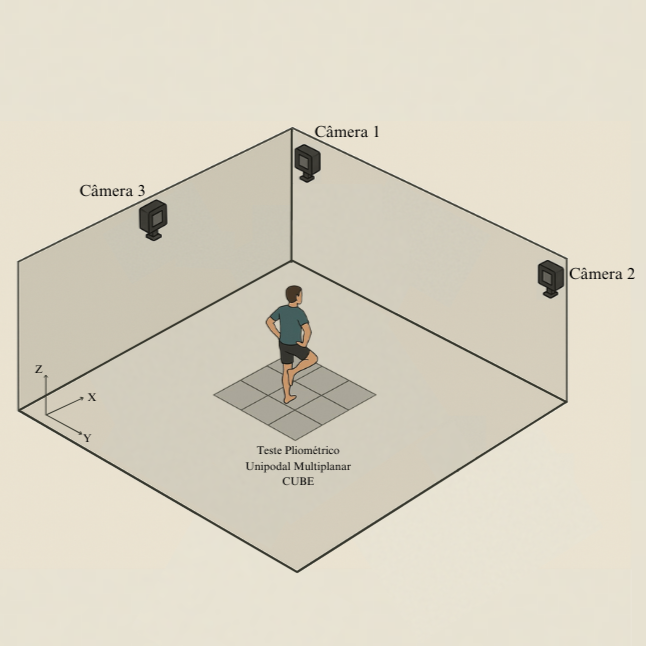
\includegraphics[width=0.35\linewidth]{images/distp_cameras.png}
    
    \small Fonte: Elaborado pelo autor (2025)
    \label{Figura 1}
\end{figure}

Será utilizado o teste CUBE (“Chameleon 360 Sports Training, Inc.”; Athens, AL), descrito como um teste pliométrico multiplanar de realização bilateral projetado para avaliação em momentos de mudanças de direção. Durante a execução, o paciente realiza uma sequência de saltos pliométricos unipodais no sentido horário e anti-horário com ambas as pernas como é possível observar na Figura \ref{Figura 2}. \\

\begin{figure} [H]
    \centering
    \caption{Referências do teste Pliométrico Unipodal Multiplanar CUBE}
    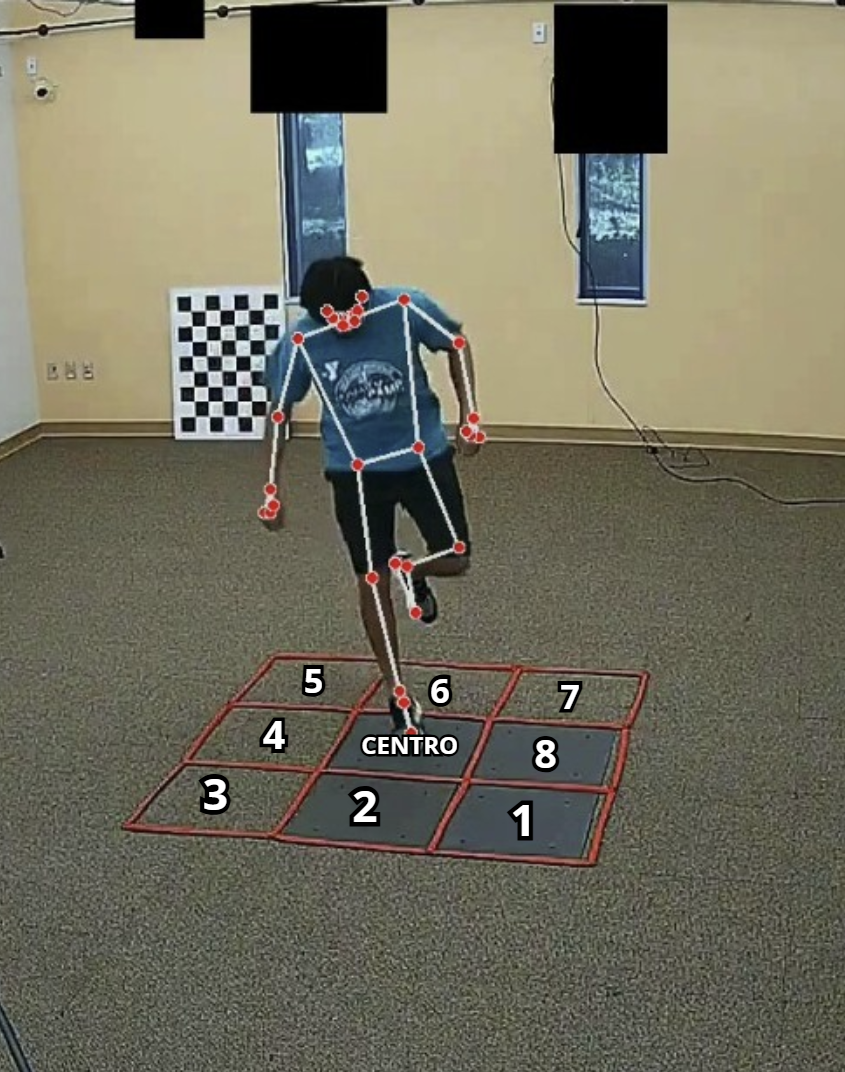
\includegraphics[width=0.3\linewidth]{images/protocol_aplication.png}
    
    \small Fonte: Elaborado pelo autor (2025)
    \label{Figura 2}
\end{figure}

Para o rastreamento cinemático e reconstrução 3D será utilizado o \textit{toolbox} multimodal \textit{\textit{MediaPipe}} \cite{google2025MediaPipe} integrado na plataforma \href{https://github.com/vaila-multimodaltoolbox/vaila}{\textit{vailá - Multimodal Toolbox}}~\cite{pereira2024vaila} a fim de realizar a construção de pipelines de Aprendizado de Máquina de forma amigável com código aberto, com foco no processamento de vídeos e imagens. As marcações terão como referências anatômicas 14 estruturas: cabeça, tronco, braços, antebraços, mãos, coxas, pernas e pés. A partir disso, 20 \textit{landmarks} serão utilizados, com base no modelo de 33 pontos anatômicos do \textit{MediaPipe}: nariz, ombros direito e esquerdo, cotovelos direito e esquerdo, punhos direito e esquerdo, pontas dos dedos indicadores direito e esquerdo, quadris direito e esquerdo, joelhos direito e esquerdo, tornozelos direito e esquerdo, calcanhares direito e esquerdo e dedões dos pés (hálux) direito e esquerdo (Figura \ref{Figura 3}). \\

\begin{figure}[H]
    \centering
    \caption{Referências anatômicas para o framework \textit{\textit{MediaPipe}}.}
    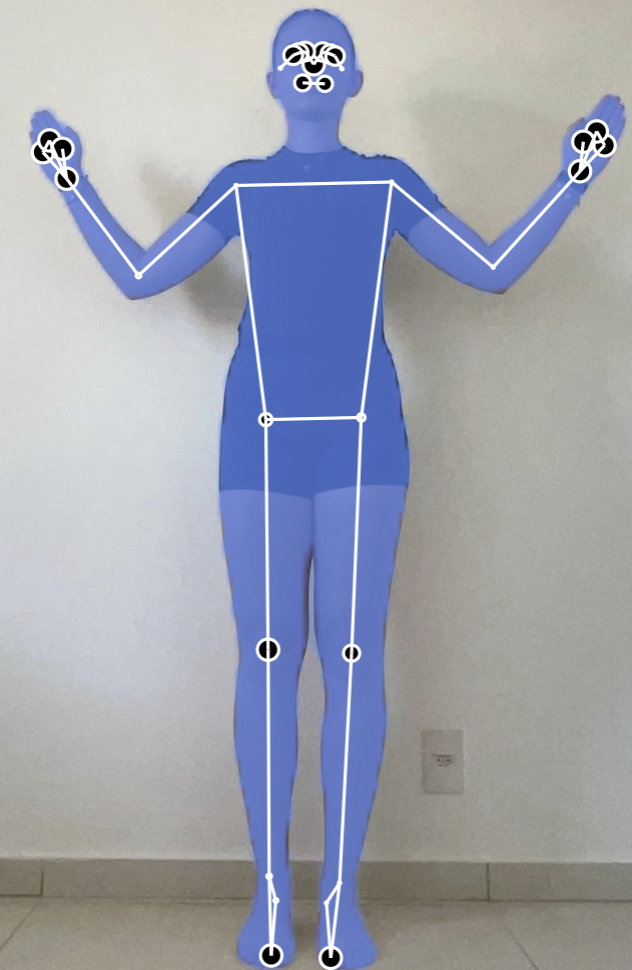
\includegraphics[width=0.25\linewidth]{images/pontos_mediapipe.png}
    
    \small{Fonte: Elaborado pelo autor (2025)}
    \label{Figura 3}
\end{figure}


\subsection{Protocolo de avaliação para os especialistas}
\noindent A avaliação subjetiva da estabilidade do joelho será conduzida utilizando métricas que consideram o risco de lesão no Ligamento Cruzado Anterior (LCA). Embora esse risco seja multifatorial, diversos estudos destacam a influência de fatores como o valgo do joelho~\cite{della2020systematic, renstrom2008non, asaeda2024reliability, hewett2005biomechanical}, a flexão do tornozelo~\cite{xu2024contribution}, e as posições do tronco, quadril e joelho~\cite{leppanen2017sagittal, blackburn2008influence} na instabilidade articular e consequente aumento no risco de lesão.

Movimentos com menor flexão articular, próximos à extensão completa, comprometem a capacidade dos segmentos de distribuir adequadamente as forças durante movimentos, que resultam na sobrecarga no joelho. Essa sobrecarga é reconhecida como um fator de alto risco para lesões do LCA~\cite{MohammadiOrangi2024}.

Instrumentos clínicos como o Single-Leg Landing Error Scoring System (SL-LESS)~\cite{padua2009landing} e o Qualitative Analysis of Single Leg Loading (QASLS)~\cite{parry2023reliability} servem como referência para a avaliação cinética do joelho, considerando variáveis mencionadas anteriormente. O SL-LESS, adaptado do LESS para saltos unipodais, visa identificar padrões de movimento associados ao risco de lesão do LCA a partir de vídeos nos planos frontal e sagital~\cite{padua2009landing}. O QASLS, por sua vez, utiliza critérios distintos para avaliar gravações de tarefas unipodais, como saltos e agachamentos~\cite{parry2023reliability}.

Os especialistas avaliadores serão 2 médicos e 2 fisioterapeutas, estes terão acesso a vídeos padronizados do teste pliométrico multiplanar CUBE, juntamente com instruções gerais do projeto. A avaliação do movimento será realizada com base em seus referenciais clínicos, focando na estabilidade articular e na qualidade do movimento, especialmente em relação aos fatores de risco previamente destacados. A partir das gravações da realização do teste pliométrico unipodal multiplanar CUBE de cada paciente disponibilizados aos profissionais, eles atribuirão às execuções scores entre 1 e 5, sendo 1 representante da baixa observação de fatores de risco de lesão do LCA e 5 a maior probabilidade de ocorrência.

Para garantir a confiabilidade dos resultados, será desenvolvido um formulário padronizado de avaliação. Serão conduzidas sessões de calibração entre os especialistas para alinhar os critérios de pontuação e minimizar a variabilidade interavaliador. A análise de concordância entre avaliadores será realizada utilizando o coeficiente Kappa de Cohen (K)~\cite{cohen1960}, que mede o grau de concordância entre observadores. Valores de K superiores a 0,8 indicam alto nível de concordância.

Além disso, as mesmas variáveis serão consideradas no desenvolvimento do modelo de Aprendizado de  Máquina, permitindo o treinamento da rede com os dados obtidos. A imagem \ref{fig:pipeline_markerless} é uma representação visual do processo de Machine Learning que será utilizado para prever o escore atribuído por cada especialista. A partir do processamento a ser realizado, portanto, a avaliação clínica será correlacionada às features biomecânicas extraídas por um sistema \textit{markerless} durante a realização do teste pliométrico unipodal multiplanar.


%Para avaliação subjetiva da establidade do joelho serão utilizadas as métricas que levam em consideração que o risco de lesão no Ligamento Cruzado Anterior. Este é multifatorial, mas diversos estudos mostram a interferência de valgo do joelho~\cite{della2020systematic, renstrom2008non, asaeda2024reliability,hewett2005biomechanical} e flexão de tornozelo \cite{xu2024contribution}, tronco, quadril e joelho \cite{leppanen2017sagittal,blackburn2008influence} na maior instabilidade articular e consequente aumento no risco de lesão. Quanto mais próximo da extensão, pior a capacidade do segmento de distribuir corretamente a força peso que age sobre a pessoa, além das forças de reação do solo por ela geradas, assim, em momentos de menores flexões articulares, o joelho pode apresentar sobrecarga, a qual é também um fator de alto risco para a lesão de LCA \cite{MohammadiOrangi2024}. 

%Ademais, o teste Single-leg Landing Error Scoring System (SL-LESS) \cite{padua2009landing} e Qualitative Analysis of Single Leg Loading (QASLS) \cite{parry2023reliability} são ferramentas que servem como base para a avaliação cinética do joelho e também consideram, entre outras, as variáveis anteriormente destacadas. O primeiro é um instrumento clínico cujo objetivo é identificar padrões de movimento associados ao risco de lesão do LCA durante tarefas de salto a partir de vídeos obtidos no plano frontal e sagital \cite{padua2009landing}. O teste original (LESS) leva em consideração saltos bilaterais, o SL-LESS, entretanto, tem o mesmo objetivo, mas utiliza-se de saltos unipodais para sua aplicação \cite{earlboehm2022slless}. De forma complementar, o segundo, usa critérios diferentes na avaliação de gravações feitas durante a realização de tarefas unipodais, como saltos e agachamentos \cite{parry2023reliability}. Os especialistas que atuarão como avaliadores terão a sua disposição os vídeos padronizados da realização do teste pliométrico multiplanar CUBE, além das instruções gerais do projeto, e realizarão a avaliação do movimento com base em seus referenciais clínicos, observando aspectos relacionados à estabilidade articular e à qualidade do movimento, em especial, no que tange os fatores de risco já apresentados. Ademais, estas variáveis serão levadas em consideração no desenvolvimendo do Aprendizado de Máquina de forma que, posteriormente, seja feita o treinamento da rede com ambos os dados obtidos.

%A presente análise busca concluir o objetivo específico 2. Para garantia da confiabildiade dos resultados obtidos, serão realizadas correlações inter-avaliadores utilizando-se do desempenho de, pelo menos, 1 amostra válida por participante. Esta terá seus resultados comparados testado pelo índice Kappa de Cohen (K)~\cite{cohen1960}. O Coeficiente Kappa pode ser definido como uma medida de associação usada para descrever e testar o grau de concordância, confiabilidade e precisão dentro de uma classificação. Ele indica alto nível de concordância para as correlações que possuem K > 0,8.

\subsection{Procedimentos experimentais}
\noindent

O teste Pliométrico Unipodal Multiplanar \textit CUBE (“Chameleon 360 Sports Training, Inc.”; Athens, AL) será aplicado a partir da delimitação de um quadrado no solo segmentado em dimensões 3x3 (cada quadrado menor com medida lateral de 0,45m) no qual o paciente realizará saltos unipodais em quatro aplicações diferentes. Na primeira, os saltos ocorrerão no sentido horário na sequência seguindo o Fluxograma 1 representado pela Figura~\ref{Figura4} a partir do modelo representado pela Figura 3. A segunda sequência é dada pela inversão do sentido de giro, seguindo a do Fluxograma 2 da Figura~\ref{Figura5}, assim, os pacientes realizarão o protocolo no sentido anti-horário. As seguintes aplicações seguem o mesmo raciocínio, entretanto, há a troca do membro com a qual realizam-se os saltos. Todos os pacientes realizarão o protocolo, inicialmente, com a perna direita. \\

\begin{figure}[H]
    \centering
    \begin{minipage}{0.45\linewidth}
        \centering
        \caption{Fluxograma CUBE - sentido horário}
        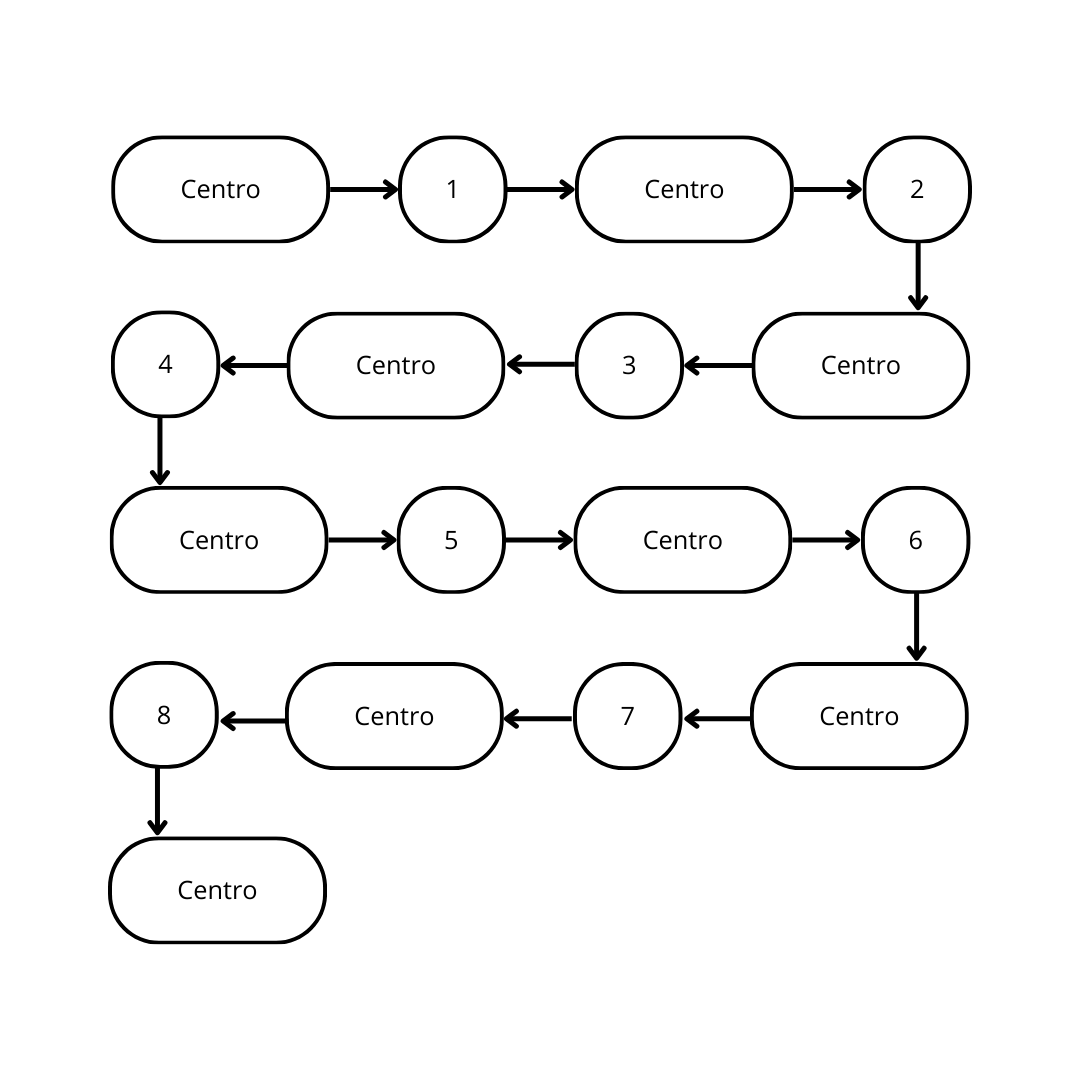
\includegraphics[width=\linewidth]{images/flux_horario.png}

        \small{Fonte: Elaborado pelo autor (2025)}
        \label{Figura4}
    \end{minipage}
    \hfill
    \begin{minipage}{0.45\linewidth}
        \centering
        \caption{Fluxograma CUBE - sentido anti-horário}
        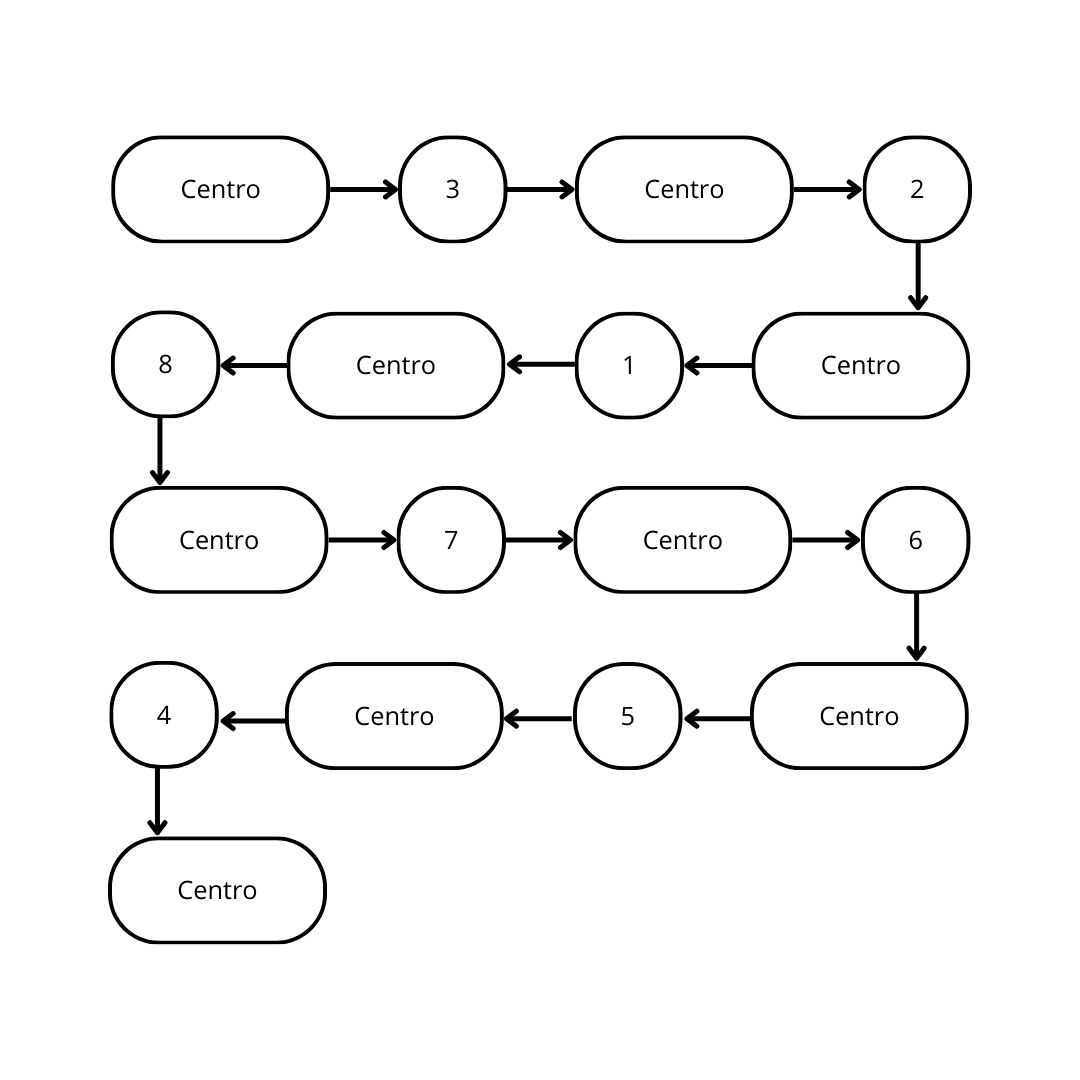
\includegraphics[width=\linewidth]{images/flux_antihorario.png}
        
        \small{Fonte: Elaborado pelo autor (2025)}
        \label{Figura5}
    \end{minipage}
\end{figure}

\subsection{Processamento de Dados}
A extração cinemática será conduzida no \emph{MediaPipe}, \emph{framework} de código aberto do Google que detecta, em tempo real, 33 pontos anatômicos no corpo humano por meio de redes neurais convolucionais. Esse sistema realiza inferência a partir de vídeos utilizando algorítmos de Aprendizado de Máquina, o que possibilita a extração automática de séries temporais bidimensionais (coordenadas $x$ e $y$) para cada articulação (Figura~\ref{Figura 2}). Cada vídeo será processado a 240 fps, gerando um conjunto de dados cinemáticos a serem analisados.%

As séries 2D obtidas serão suavizadas por filtro Butterworth de quarta ordem, com frequência de corte definida pela análise de resíduos \cite{Winter2009}. Posteriormente, aplicaremos a Transformação Linear Direta 3D (3D‑DLT) para reconstruir as coordenadas no espaço global, utilizando um volume calibrado por nove marcadores estáticos posicionados no ambiente antes da coleta. Esse processo permitirá a obtenção de coordenadas 3D confiáveis, que serão utilizadas para o cálculo de variáveis cinemáticas.%

Com as coordenadas filtradas e reconstruídos, calcularemos automaticamente variáveis discretas que descrevem o desempenho no CUBE. O ciclo de salto será definido pelo intervalo entre o momento em que o pé de apoio abandona o quadrado central pela primeira vez e o instante em que retorna a essa posição pela última vez. Nos instantes de contato em cada quadrado, identificaremos o pico de flexão de tornozelo, joelho e quadril, bem como a máxima projeção do tronco. Em seguida, scripts de verificação visual conferem coerência biomecânica dos ângulos.%

O processamento de vídeos e o desenvolvimento dos modelos de aprendizado de máquina serão executados por pesquisadores cegos quanto ao lado lesado, minimizando viés de confirmação durante o treinamento, a validação e a interpretação dos resultados. Essa abordagem garante maior confibilidade aos achados, mantendo a integridade do processo analítico.%

\subsection{Conjunto de Dados e Variáveis}
Antes da modelagem, organizamos as variáveis em quatro blocos, descrevendo abaixo a lógica de cada grupo. Essa separação guiará tanto a análise estatística quanto a seleção de preditores.%

\subsubsection{CUBE –– Métricas Espaço‑Temporais 2D}
Os parâmetros básicos resumem a cinemática global da tarefa e serão usados como covariáveis de contexto.%
\begin{itemize}
    \item \textbf{Distância total, velocidade média e velocidade máxima};
    \item \textbf{Tempo parado, tempo total e percentagem de movimento (\%mov)}. \\
    Calculado como: $\%mov = 100 \times (\text{tempo em deslocamento} \/ \text{tempo total})$
\end{itemize}



\subsubsection{Variáveis 2D Projetadas}
Estas métricas são obtidas diretamente do plano da câmera frontal e exigem apenas pose 2D.%
\begin{itemize}
    \item Dynamic Knee Valgus (instante de contacto e pico);
    \item Frontal Plane Projection Angle (FPPA);
    \item Inclinação pélvica 2D (\emph{pelvic tilt});
    \item Inversão/Eversão de tornozelo (pico);
    \item Inclinação lateral de tronco;
    \item Tempo de contacto (GCT) e tempo de voo.
\end{itemize}

\subsubsection{Variáveis 3D Articulares e do Centro de Massa}
Reconstruídas por 3D‑DLT, descritas em momentos‑chave (IC, pico de flexão, decolagem).%

\begin{itemize}
    \item Ângulo de abdução/valgo do joelho;
    \item Rotação interna do joelho;
    \item Flexão, adução e rotação do quadril;
    \item Dorsiflexão do tornozelo;
    \item Obliquidade pélvica (\emph{drop}) e \emph{tilt} sagital;
    \item Velocidade vertical e deslocamento máximo do centro de massa (CoM);
    \item Extrapolated Center of Mass (XCoM).
\end{itemize}

\subsubsection{Variáveis de Coordenação (Vector Coding)}
Obtidas pela técnica de \emph{vector coding}, descrevem como os segmentos interagem.%

\begin{itemize}
    \item Hip–Knee Coupling Angle (\% \emph{in‑phase} vs. \emph{anti‑phase});
    \item Knee–Ankle Coupling Angle;
    \item Variabilidade de acoplamento (desvio‑padrão do ângulo).
\end{itemize}

\subsubsection{Variáveis Temporais Normalizadas}
Expressas em milissegundos e normalizadas pela duração total do salto.%

\begin{itemize}
    \item Tempo até pico de flexão do joelho;
    \item Tempo até pico de valgo;
    \item
        Índice de fadiga (diferença entre o tempo de contacto inicial até o tempo do pico de flexão do joelho). A fórmula utilizada é:
        
    \colorbox{white}{%
        \parbox{\dimexpr\linewidth-2\fboxsep}{%
        \[
        \text{Índice de Fadiga} = \frac{(t_{\text{pico}} - t_{\text{IC}})_{\text{final}} - (t_{\text{pico}} - t_{\text{IC}})_{\text{inicial}}}{(t_{\text{pico}} - t_{\text{IC}})_{\text{inicial}}} \times 100\%
        \]
}}
    \item Esse índice reflete alterações temporais nos eventos de aterrissagem ao longo da tarefa, podendo indicar efeitos de fadiga neuromuscular.
\end{itemize}

%A fórmula utilizada é:
%\begin{equation}
%    \text{Índice de Fadiga} = \frac{(t_{\text{pico}} - t_{\text{IC}})_{\text{final}} - (t_{\text{pico}} - t_{\text{IC}})_{\text{inicial}}}{(t_{\text{pico}} - t_{\text{IC}})_{\text{inicial}}} \times 100\%
%\end{equation}
%Esse índice reflete alterações temporais nos eventos de aterrissagem ao longo da tarefa, podendo indicar efeitos de fadiga neuromuscular.



















\subsection{Aprendizado de Máquina}
\noindent Este estudo visa atender ao Objetivo Específico 4 por meio da aplicação de técnicas de Aprendizado de Máquina supervisionado, com o propósito de prever a avaliação funcional subjetiva atribuída por especialistas a pacientes com lesão do Ligamento Cruzado Anterior. A predição será realizada com base na análise de variáveis cinemáticas extraídas durante a execução do teste Pliométrico Unipodal Multiplanar CUBE. Conforme descrito no tópico 4.3 deste projeto, essas variáveis estão associadas ao aumento do risco de lesão do LCA e incluem: valgo do joelho, flexão de tronco, flexão de quadril, de joelho e de tornozelo.

Para o desenvolvimento dos modelos preditivos, será utilizada a biblioteca \textit{Scikit-learn}, uma ferramenta de código aberto em Python amplamente adotada para tarefas de aprendizado de máquina supervisionado, incluindo classificação, regressão e agrupamento~\cite{scikit-learn}. A \textit{Scikit-learn} fornece uma interface consistente e eficiente para a implementação de diversos algoritmos de classificação, facilitando a experimentação e comparação de modelos.

Serão avaliados e comparados os desempenhos dos seguintes algoritmos de classificação supervisionada:

\begin{enumerate}
    \item \textbf{Extreme Gradient Boosting (XGBoost)}: um algoritmo de aprendizado de máquina baseado em árvores de decisão, conhecido por sua eficiência e desempenho em competições de ciência de dados~\cite{chen2016xgboost}.
    \item \textbf{Random Forest}: um método de ensemble que constrói múltiplas árvores de decisão e as combina para obter uma previsão mais precisa e estável~\cite{breiman2001random}.
    \item \textbf{Regressão Logística}: um modelo estatístico que utiliza uma função logística para modelar a probabilidade de uma determinada classe ou evento~\cite{hosmer2013applied}.
    \item \textbf{K-Nearest Neighbors (KNN)}: um algoritmo que classifica uma amostra com base nas classes dos seus vizinhos mais próximos no espaço de características~\cite{cover1967nearest}.
    \item \textbf{Support Vector Machine (SVM)}: um modelo que encontra o hiperplano ótimo que separa as classes no espaço de características, sendo eficaz em espaços de alta dimensão~\cite{cortes1995support}.
    \item \textbf{Gaussian Naive Bayes}: um classificador probabilístico baseado no Teorema de Bayes, assumindo independência entre as características~\cite{rish2001empirical}.
    \item \textbf{Perceptron Multicamadas (MLP)}: uma rede neural \textit{feedforward} composta por múltiplas camadas de neurônios, capaz de modelar relações não lineares complexas~\cite{rumelhart1986learning}.
\end{enumerate}

É importante ressaltar que, embora técnicas de Aprendizado de Máquina geralmente requeiram grandes volumes de dados para uma generalização eficaz dos modelos, este estudo enfrenta limitações como o tempo disponível para coleta e análise de dados, além de se tratar de um projeto de iniciação científica. Consequentemente, a amostra obtida pode não representar plenamente a complexidade necessária para a construção de modelos altamente generalizáveis. No entanto, este estudo constitui uma etapa inicial que poderá ser expandida e aprofundada em futuras investigações, com a inclusão de um volume maior de dados e, consequentemente, o aprimoramento dos modelos preditivos desenvolvidos.


%A aplicação \cite{Taylor2020} de técnicas de Aprendizado de Máquina buscará responder ao objetivo específico 3. A predição da avaliação subjetiva dos especialistas será feita por meio da análise das variáveis cinemática de desempenho do teste Pliométrico Unipodal Multiplanar CUBE mediada pelas referências dadas na Tabela \ref{Tabela 1}. Serão utilizados modelos de Aprendizado de Máquina supervisionado para classificação. Para isso, será utilizada a biblioteca de Aprendizado de Máquina em Python, a Scikit-learn. Será comparado o desempenho de 7 modelos de Aprendizado de Máquina utilizados para classificação: Extreme Gradient Boosting algorithm, Random Forest, Logistic Regression, K-nearest neighbors, Support Vector Machine, Gaussian Naive Bayes e Multilayer Perceptron. 

%É importante destacar que, embora técnicas de Aprendizado de Máquina geralmente demandem grandes volumes de dados para generalização dos modelos, o presente estudo possui limitações, tais como o tempo disponível para coleta e análise de dados, além de se tratar de um projeto de iniciação científica. Assim, a amostra obtida poderá não representar plenamente a complexidade necessária para a construção de modelos. Entretanto, este estudo configura-se como uma etapa inicial, que poderá ser ampliada e aprofundada em futuras investigações, com a inclusão de um volume maior de dados e, consequentemente, o aprimoramento das redes preditivas desenvolvidas.

\subsubsection{Pré-Processamento}

\noindent As variáveis cinemáticas extraídas do teste CUBE serão organizadas e combinadas para a construção dos conjuntos de dados utilizados como preditores nos modelos de aprendizado de máquina. As variáveis serão normalizadas utilizando o \textit{StandardScaler} da biblioteca Scikit-learn, garantindo média zero e variância unitária em cada feature.

A seleção e otimização dos hiperparâmetros dos modelos será realizada por meio da técnica \textit{Grid Search}, adotando como critério principal a acurácia balanceada obtida nos conjuntos de validação. Para garantir que a proporção das classes seja mantida em todas as partições, será utilizada a técnica \textit{StratifiedKFold} durante a validação cruzada, assegurando a representatividade das classes minoritárias e maior robustez na avaliação dos modelos.

Para garantir a reprodutibilidade dos experimentos, será utilizado um valor fixo de \textit{random\_state} em todas as divisões dos dados. A validação cruzada será repetida 30 vezes, empregando diferentes divisões aleatórias, a fim de reduzir a variabilidade dos resultados e fornecer uma avaliação robusta do desempenho dos modelos.




\subsubsection{Avaliação dos Modelos}

\noindent A avaliação dos modelos de aprendizado de máquina será conduzida utilizando as seguintes métricas: acurácia balanceada (\textit{balanced accuracy}), precisão (\textit{precision}), sensibilidade (\textit{recall}) e F1-Score. Essas métricas serão calculadas tanto individualmente para cada classe quanto para a média geral (\textit{macro average}), permitindo uma análise abrangente do desempenho dos modelos em diferentes cenários de classificação.

Será selecionada, ao final, a combinação de variáveis cinemáticas e hiperparâmetros que apresentar o melhor desempenho em acurácia balanceada para a predição da avaliação funcional atribuída pelos especialistas. A partir dessa abordagem, busca-se identificar padrões de movimento que contribuem de forma significativa para a predição do estado de estabilidade do joelho dos pacientes avaliados durante o teste CUBE.

A Figura \ref{fig:pipeline_markerless} sintetiza todo o fluxo analítico empregado neste estudo, desde a reconstrução \textit{markerless} da pose humana até a geração do escore clínico previsto. O diagrama evidencia a sequência lógica das etapas: (i) extração automática das coordenadas 2D e 3D com ferramentas de visão computacional; (ii) formação do dataset de variáveis cinemáticas; (iii) pré-processamento, incluindo normalização e engenharia de atributos; (iv) treinamento de múltiplos algoritmos supervisionados; (v) avaliação por meio das métricas descritas nesta subseção; e, por fim, (vi) comparação com a avaliação funcional de referência fornecida pelos especialistas.

Ao alinhar cada bloco do organograma com as fases descritas no texto, assegura-se que o procedimento estatístico esteja completamente rastreável, o que fortalece a reprodutibilidade do protocolo e facilita futuras extensões do estudo.

%\subsubsection{Pré-Processamento}
%As variáveis cinemáticas do CUBE serão combinadas para criar diferentes conjuntos de dados como variáveis preditoras, normalizadas usando o StandardScaler, Grid Search e Validação Cruzada. O Grid Search será utilizado para otimizar os hiperparâmetros dos modelos, escolhendo a melhor combinação com base na acurácia balanceada. A técnica StratifiedKFold será usada para manter a proporção das classes em cada subdivisão dos dados, e um valor fixo de Random State garantirá a reprodutibilidade dos resultados. A validação cruzada será executada 30 vezes, com a técnica de divisão aleatória com diferentes valores em cada execução, para garantir uma avaliação mais robusta dos modelos.

%\subsubsection{Avaliação dos Modelos}
%As métricas escolhidas para avaliação dos modelos serão acurácia balanceada, precisão, recursão, e F1 Score. Essas métricas serão reportadas tanto para cada uma das 4 classe quanto para a média geral. Será selecionada a combinação de variáveis cinemáticas com melhores valores de acurácia balanceada para predição da avaliação subjetiva dos especialistas, identificando, dessa forma, através da realização do teste CUBE, padrões de movimento responsáveis pela predição do estado de establididade do joelho dos pacientes.



%-------------------------------------------------------------
% Fluxograma do pipeline – legendas acima, formato completo
%-------------------------------------------------------------
% Requisitos no preâmbulo:
% \usepackage{tikz}
% \usetikzlibrary{positioning, arrows.meta}
%-------------------------------------------------------------
\begin{figure}[H]
    \centering
    % ---- caption acima da ilustração ----
    \caption{Pipeline completo: vídeos são processados via CV com \emph{markerless} para reconstruir a pose 2D/3D. As variáveis cinemáticas alimentam modelos de ML/DL que predizem o escore clínico (1--5).}

    % ---- diagrama TikZ ----
    \begin{tikzpicture}[
        scale=0.85, transform shape, % << redução aplicada aqui
        node distance = 1.3cm and 1.0cm,
        base/.style   ={rounded corners, draw=black, font=\sffamily\small,
                        align=center, minimum width=6cm, minimum height=1.4cm},
        markerless/.style={base, fill=purple!15},
        dataset/.style   ={base, fill=blue!15},
        preprocess/.style={base, fill=gray!15},
        training/.style  ={base, fill=green!15},
        evaluation/.style={base, fill=white!20},
        score/.style     ={base, fill=red!20, rotate=90, minimum width=4cm,
                           minimum height=1.4cm},
        arrow/.style={-Stealth, thick}
    ]

    % --- nós ---
    \node[markerless] (cv) {\textbf{Markerless CV}\\Pose Estimation 2D \& 3D\\(MediaPipe)};

    \node[dataset, below=of cv] (data) {\textbf{Dataset de Features}\\27 variáveis + Target\\DKV, FPPA, CoM, Vector Coding, $\dots$};

    \node[preprocess, below=of data] (prep) {\textbf{Preprocessing}\\Cleaning – Normalization – Engineering};

    \node[training, below=of prep] (train) {\textbf{Model Training}\\SVM, RF, XGBoost, MLP,\\CNN, LSTM, Autoencoder};

    \node[evaluation, below=of train] (eval) {\textbf{Model Evaluation}\\Accuracy, F1, Confusion Matrix};

    \node[score, right=2.7cm of train] (score) {\textbf{Expert Score}\\(1--5)};

    % --- setas ---
    \draw[arrow] (cv)   -- (data);
    \draw[arrow] (data) -- (prep);
    \draw[arrow] (prep) -- node[left]{\small Train/Test Split} (train);
    \draw[arrow] (train) -- (eval);
    \draw[arrow] (train) -- (score);

    \end{tikzpicture}

    % ---- fonte/nota ----
    \small Fonte: Elaborado pelo autor (2025)

    \label{fig:pipeline_markerless}
\end{figure}





\subsection{Análise estatística}

\noindent As métricas de desempenho dos modelos de Aprendizado de Máquina, bem como os valores das variáveis cinemáticas extraídas do teste Pliométrico Unipodal Multiplanar CUBE, serão descritos por meio de média e desvio padrão. As comparações serão realizadas entre os modelos com melhor desempenho e entre os diferentes momentos de avaliação dos participantes.

A verificação da normalidade dos dados será conduzida utilizando o teste de Shapiro-Wilk, enquanto a homogeneidade das variâncias será avaliada pelo teste de Levene. Em casos onde os dados apresentarem distribuição normal e variâncias homogêneas, será aplicada a análise de variância unidirecional (ANOVA one-way), seguida do teste post-hoc de Tukey HSD (Honestly Significant Difference) para comparações múltiplas.

Quando as suposições de normalidade ou homogeneidade não forem atendidas, será utilizado o teste não paramétrico de Kruskal-Wallis, seguido do teste post-hoc de Dunn com ajuste de Bonferroni para comparações entre grupos. O tamanho do efeito para cada comparação será estimado pelo d de Cohen.

O nível de significância adotado para todas as análises será de $p < 0{,}05$. Todas as análises estatísticas serão realizadas utilizando códigos em Python 3.12.11, empregando as bibliotecas \texttt{SciPy} \cite{2020SciPy-NMeth}, \texttt{statsmodels} \cite{seabold2010statsmodels} e \texttt{scikit-posthocs} \cite{terpilowski2019scikit}.

%Tanto as métricas descritas na sessão avaliação dos modelos de Aprendizado de Máquina quanto os valores das variáveis cinemáticas do teste Pliométrico Unipodal Multiplanar CUBE serão descritos em média e desvio padrão e comparados entre os melhores modelos e entre os diferentes momentos da avaliação. A normalidade e homogeneidade serão verificadas pelos testes de Shapiro-Wilk e Levene. Quando os dados apresentaram distribuição normal e homogênea, eles serão comparados utilizando a Anova one-way e o post-hoc de Tukey's HSD (Honestly Significant Difference). Quando a distribuição dos dados não for normal e homogênea, as métricas serão comparadas utilizando o teste de Kruskal-Wallis com post-hoc de Dunn com ajuste de Bonferroni. Para descrição do tamanho de efeito será calculado o d de Cohen para cada comparação. Em todos os casos o nível de significância considerado será de p<0,05. As análises serão realizadas por meio de algoritmos em Python 3. 

\section{Relatório de Atividades Realizadas (Situação Atual)}

\noindent Até o presente momento, o projeto apresenta os seguintes avanços e resultados preliminares:

\begin{enumerate}
    \item \textbf{Coleta de Dados}: Foram realizadas com sucesso 6 sessões de coleta de dados cinemáticos com pacientes entre 6 e 8 meses de pós-operatório de reconstrução de LCA. Apesar de algumas desistências pontuais, o recrutamento continua ativo para atingir a meta amostral.
    \item \textbf{Infraestrutura e Padronização}: O ambiente de coleta no consultório colaborador foi devidamente calibrado utilizando marcadores estáticos e as três câmeras GoPro Hero 10 sincronizadas.
    \item \textbf{Processamento de Vídeo}: A pipeline inicial de Visão Computacional (\textit{MediaPipe}) e reconstrução 3D (\textit{DLT}) foi testada e validada com as primeiras amostras.
    \item \textbf{Internacionalização (BEPE)}: O planejamento para o estágio de pesquisa no exterior (\textit{University of North Florida}) está concluído. A aluna já recebeu a carta de convite oficial para o período de junho a dezembro de 2026, focando na validação transcultural do modelo.
    \item \textbf{Conformidade Ética}: Todas as atividades seguem rigorosamente o protocolo aprovado (CAAE 89943725.2.0000.5659).
\end{enumerate}

\section {Atividades a serem desenvolvidas pelo bolsista}
\begin{itemize}
    \item Agendar e filmar sessões; organizar metadados.
    \item Executar scripts de pose estimation para extrair séries 2D e 3D.
    \item Análise exploratória e correlações em código Python.
    \item Criar e desenvolver \textit{template} para treinar cada algoritmo; selecionar hiper parâmetros via busca bayesiana.
    \item Elaborar resumo científico.
\end{itemize}

\section{Cronograma}

\noindent O cronograma apresentado distribui as principais etapas do projeto ao longo de doze meses, organizando desde a capacitação da aluna, recrutamento e coleta de dados, tratamento de dados e treinamento do modelo, comparação estatística com avaliação clínica e finalização com a redação científica e relatório final. Essa sequência garante que cada etapa seja conduzida de forma estruturada, favorecendo o alcance dos objetivos do estudo dentro do prazo previsto.

Ressalta-se que, embora o cronograma esteja ajustado em 12 meses para atender à norma vigente da FAPESP/CNPq/PUB-USP para bolsas de Iniciação Científica, determinadas etapas do projeto poderão, na prática, estender-se além desse período, conforme a necessidade de execução e acompanhamento dos participantes.

O projeto conta com a colaboração do médico Dr.~\href{http://lattes.cnpq.br/3097142727488536}{Rodrigo Salim}, coorientador e parte interessada direta na pesquisa, responsável pelo convite e encaminhamento dos pacientes para as avaliações. Dada sua reconhecida experiência profissional e acadêmica, sua atuação é fundamental para o sucesso do projeto, assegurando rigor clínico no processo de seleção e acompanhamento dos participantes.

Como colaborador doutorando, participa \href{http://lattes.cnpq.br/7197039502542262}{Rafael Luiz Martins Monteiro}, que contribuirá ativamente no desenvolvimento experimental, análise dos dados e discussão dos resultados, ampliando a integração entre diferentes níveis de formação acadêmica e fortalecendo o caráter multidisciplinar da pesquisa.

Além disso, o projeto conta com a colaboração internacional do pesquisador Dr.~\href{https://webapps.unf.edu/faculty/bio/N01526872}{Guilherme Manna Cesar}, da University of North Florida. Sua atuação é especialmente relevante para o planejamento de futuras experiências de internacionalização, como a realização de um estágio BEPE, ampliando as oportunidades de troca acadêmica, colaboração científica e enriquecimento da formação dos envolvidos no projeto. \\



\begin{table}[h!]
\centering
\caption{Cronograma de atividades}
\label{tab:cronograma_destacado} % Adicionei um label para referência
\begin{tabular}{
>{\raggedright\arraybackslash}m{8cm} % Coluna para as atividades
*{12}{c} % 12 colunas para os meses, centralizadas
}
\toprule
\rowcolor{white} % Destaca a primeira linha de cabeçalho
\textbf{Atividades} & \multicolumn{12}{c}{\textbf{Meses para realização}} \\
\cmidrule(lr){2-13} % Linha horizontal parcial
\rowcolor{white} % Destaca a segunda linha de cabeçalho
& \textbf{1} & \textbf{2} & \textbf{3} & \textbf{4} & \textbf{5} & \textbf{6} & \textbf{7} & \textbf{8} & \textbf{9} & \textbf{10} & \textbf{11} & \textbf{12} \\
\rowcolor{white} % Destaca a linha da atividade
Capacitação em processamento de vídeo e Machine Learning & \cellcolor{gray!30} & \cellcolor{gray!30} & & & & & & & & & & \\
\rowcolor{white} % Destaca a linha da atividade
Recrutamento e coleta de dados & & & \cellcolor{gray!30} & \cellcolor{gray!30} & \cellcolor{gray!30} & \cellcolor{gray!30} & & & & & & \\
\rowcolor{white} % Destaca a linha da atividade
Tratamento dos dados e treinamento do modelo & & & & & & & \cellcolor{gray!30} & \cellcolor{gray!30} & \cellcolor{gray!30} & & & \\
\rowcolor{white} % Destaca a linha da atividade
Comparação estatística com avaliações clínicas & & & & & & & & & & \cellcolor{gray!30} & \cellcolor{gray!30} & \\
\rowcolor{white} % Destaca a linha da atividade
Redação do artigo e relatório final      & & & & & & & & & & & & \cellcolor{gray!30} \\
\bottomrule
\end{tabular}
\end{table}


\newpage
%\bibliographystyle{plain}
\bibliographystyle{unsrt}
\bibliography{referencias}

\newpage
\begin{appendices}
\section{Carta de Convite - University of North Florida (UNF)}
\label{apice:carta_unf}
Abaixo, inclui-se a Carta de Convite oficial emitida pela \textit{University of North Florida}, assinada pela Dra. Sherry O. Pinkstaff e pelo Prof. Dr. Guilherme Manna Cesar.

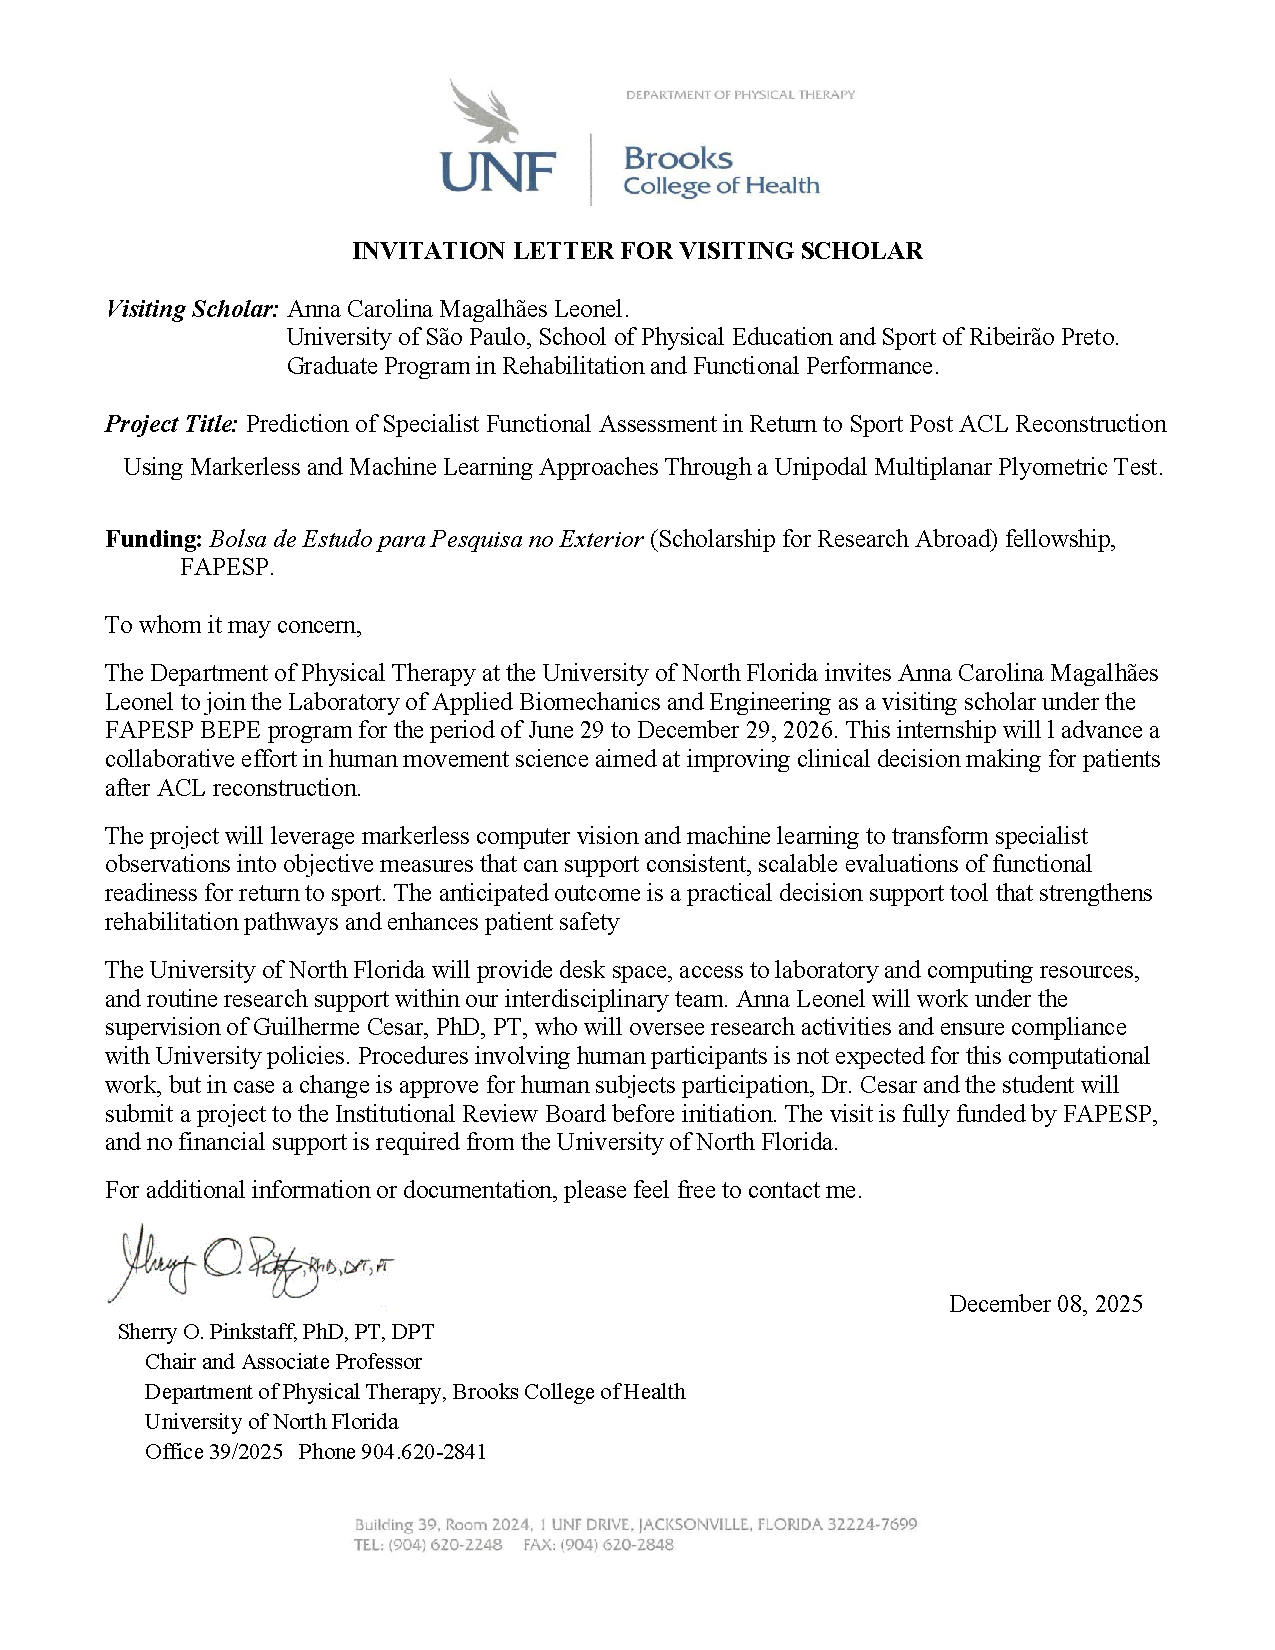
\includepdf[pages=-]{pdf/Invitation_Letter_FAPESP_BEPE_Anna_Leonel.pdf}
\end{appendices}

\end{document}


\begin{comment}

\begin{table}[h!]
\centering
\caption{Cronograma de atividades}
\begin{tabular}{
>{\raggedright\arraybackslash}m{8cm} 
*{12}{c}
}
\toprule
\rowcolor{white}
\textbf{Atividades} & \multicolumn{12}{c}{\textbf{Meses para realização}} \\
\cmidrule(lr){2-13}
\rowcolor{white}
 & \textbf{1} & \textbf{2} & \textbf{3} & \textbf{4} & \textbf{5} & \textbf{6} & \textbf{7} & \textbf{8} & \textbf{9} & \textbf{10} & \textbf{11} & \textbf{12} \\
\rowcolor{white}
Capacitação em processamento de vídeo e Machine Learning     & \cellcolor{gray!30} & \cellcolor{gray!30} &  &  &  &  &  &  &  &  &  &  \\
\rowcolor{white}
Recrutamento e coleta de dados                 &  &  & \cellcolor{gray!30} & \cellcolor{gray!30} & \cellcolor{gray!30} & \cellcolor{gray!30} &  &  &  &  &  &  \\
\rowcolor{white}
Tratamento dos dados e treinamento do modelo   &  &  &  &  &  &  & \cellcolor{gray!30} & \cellcolor{gray!30} & \cellcolor{gray!30} &  &  &  \\
\rowcolor{white}
Comparação estatística com avaliações clínicas &  &  &  &  &  &  &  &  &  & \cellcolor{gray!30} & \cellcolor{gray!30} &  \\
\rowcolor{white}
Redação do artigo e relatório final            &  &  &  &  &  &  &  &  &  &  &  & \cellcolor{gray!30} \\
\bottomrule
\end{tabular}
\end{table}
\end{comment}


